%\title{Some story wot I wrote}
\newcommand{\protagonist}{Millar}
\newcommand{\razordoc}{Dr. Stellar}

%\documentclass{article}
%\begin{document}
%\maketitle

%\paragraph{}
%The protagonist of this story, \protagonist{} (pronounced mill-AH), is agender. Ze uses ze/zir as pronouns (in place of he/him, she/her or they/them).


\footnotetext[1]{The protagonist of this story, \protagonist{} (pronounced mill-AH), is agender. Ze uses ze/zir as pronouns (in place of he/him, she/her or they/them).}

%\paragraph{Once Upon a Midnight Dreary}


\textbf{\razordoc{}}

In front of \protagonist{} was a disused warehouse. To a passerby who wasn't in the know, it would probably appear identical to any one of the many disused warehouses along this street, but \protagonist{} knew better. In reality, it was a clinic run by a razordoc, \razordoc{}.\\
Most doctors would refuse to do the kind of surgery that \protagonist{} put zirself\footnotemark[1] through. Maybe, ze mused, it was because they were afraid of what ze could become. Of how much more ze could become.\\
They claimed it was for safety, licensing or some other garbage, but \protagonist{} knew better. In general, razordocs played relatively fast and loose with the law when it came to such situations. So why would the care so much about zir safety?\\
No, the truth was that they were afraid of zir.

Still, \razordoc{} was not one of those doctors. She was even more open than most of these doctors, willing to do any job for the right money, regardless of legality. That made her the perfect doctor for someone like \protagonist{}. All ze had to do was keep the credsticks coming, and the good doctor would be more than happy to oblige.\\
Although ze hadn't checked the credsticks, \protagonist{} was pretty sure that the money on them would pay for something fun. Or, at least, something interesting.\\
Ze gave the secret knock that alerted \razordoc{} that a customer and not a random passerby was entering, before opening the door and stepping inside.

The clinic was a run-down but fairly clean and tidy affair. Much what you would expect from a good razordoc. It could be a little disorientating getting from the warehouse entrance to the reception at times, but that was the price paid for security.\\
\protagonist{} reached the reception and put zir stolen credsticks on the table.\\
``\razordoc{}. How much can I get?"\\
``\protagonist{}! Good to see you again!" The doctor was charismatic, trying to keep zir at ease. Ze wished she wouldn't. It was such a pain to hear the same, boring conversation over and over again. ``How are you? How's the... Wait, do you even have any family?"\\
``We do this every time, doctor. Can we skip the pleasantries for once? I have cash, you have cyber. What can I get?"

A little disoriented, \razordoc{} nevertheless seemed to bounce back quickly.
``Of course, sorry! Let me have a look... Hmm, it seems like there's not too much here, I'm afraid. What were you looking for, anyway?"\\
``A gun."\\
``Ah, implanted gun, very nice but also very expensive I'm afraid. This could certainly cover the surgery, but you would have to find your own implant."\\
``I can do that. I'll be back soon."\\
As \protagonist{} turned to leave, \razordoc{} called after zir.
``Don't you want your cred back?"\\
``I'll be back soon."

\begin{figure}[h!]
\centering
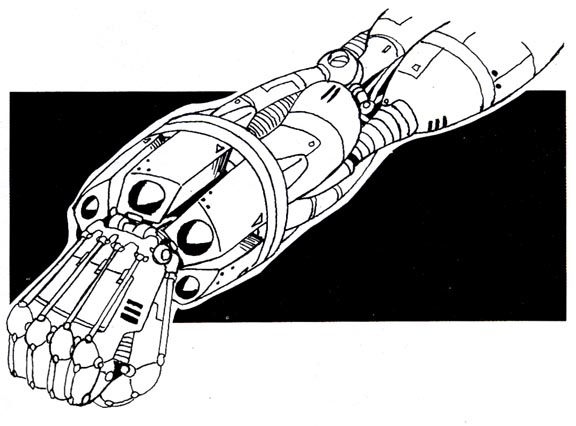
\includegraphics[width=0.7\textwidth]{./pictures/grebo-guru_arm}
\end{figure}

\textbf{Is that a Gun in Your Pocket?}

Where to start looking? \protagonist{} wanted some serious firepower, not some pea-shooter that ze could find on any street corner. And to get one that could be implanted... That would take some doing.\\
Where else, then, but the military garrison a few miles down the road? People would probably call zir crazy for even trying it... But since when did ze care what other people thought?\\
\protagonist{} took off down the street at a run, just a blur to the naked eye.

Since ze was on a mission, \protagonist{} was running almost as fast as zir augmented legs would allow. Therefore, it took merely ten minutes to reach the garrison. In the meantime, ze downloaded the plans to the complex into zir headware and planned an attack.\\
It would, of course, be ridiculous to attack the front gate. This was one time that \protagonist{} wanted to get in and out as silently as possible.\\
Rather useful, then, that the plans revealed an unused side entrance. This would probably have at least cameras and maybe even a guard or two checking it, but they would be much easier to take care of than the forces that would be guarding any other entrance.\\
It was, additionally, a simple enough route to R\&D - the most likely place to find some interesting cyberweapons...

The entrance was quiet. A knife thrown in the right direction, targeting dealt with by \protagonist{}'s headware, took out the power to the cameras. One guard was on duty, and he didn't notice a thing as \protagonist{} slipped through the shadows to end up behind him. Ze choked him out and stole his ID.\\
As expected, the R\&D lab was close by. Although the ID card that ze had stolen didn't allow zir entrance to the lab, a friend was on call to help...\\
``Johnny Mercury? \protagonist{} here." Ze called over zir commlink.\\
``You can call me Mercs like everyone else, you know."\\
``Whatever. Those plans were good, but now I need into a door."\\
``You didn't get an ID from some schmuck?" Humans were always second-guessing zir. Of course ze had an ID, it didn't have access!\\
``Too high security for that. I need your help." Sadly, this was not \protagonist{}'s area of expertise.\\
``Okay, but that's another 5k you owe me. And you'd better not get me caught up in whatever crazy plot you've got going on!"\\
``Sure. In your account now." \protagonist{} sent over the money.\\
A few seconds later, the door clicked open. He wasn't cheap, but Johnny Mercury was one fast decker.

The lab was surprisingly large. This late there were few people around, but the telltale signs of life and work were all around. Scattered pens and paper, various medical-looking instruments, computer terminals blinking... Clearly a lot was going on here.\\
There were a few credsticks on a nearby desk. \protagonist{} pocketed whatever ze saw.
Then ze heard a voice. Quickly, ze hid behind a nearby desk and watched.\\
It looked as though a few techs had stayed behind to test something. They were standing by a desk next to what was clearly some kind of testing room - testing what, though, was unclear from zir angle.\\
Ze quickly stole up behind the two techs and grabbed one neck in each hand. The two were dead before they hit the ground. Now ze could see what was going on.\\
And ze quickly regretted it.\\
Looking back through the, sadly, two-way glass was a cybersoldier. Her hand had flipped down, revealing a small minigun which she had apparently been testing on the firing range. It slowly started to spin as the soldier's expression hardened.

\protagonist{} ducked under the desk, hearing the glass shatter above zir. When the sound of bullets stopped, ze jumped over the desk, through the broken window and into the soldier.\\
She brought a knife up to bear. ``DIE!"\\
Fear was starting to get to \protagonist{}. Time to activate zir adrenal implants, which stop ze from having to worry about these annoying human emotions. Dodging out of the way of the knife, ze brought zir own out - a blade that extended from zir arm.\\
Blood spurted from a wound in the soldier's arm as \protagonist{} slashed at her.\\
``You goddamn fragging PIG!"\\
\protagonist{} was glad not to have to deal with these human emotions any more. They often got in the way.\\
One more well-placed cut was all it took to sever the gun arm from the soldier. Grabbing it, ze made a hasty retreat before more soldiers turned up. One-on-one ze was in a strong position, but too many more and it would be curtains for zir.

Slipping out the way ze came, \protagonist{} lost the soldier quickly. The streets were a good place to hide.

\textbf{Under the Knife}

\protagonist{} approached the run-down, disused warehouse that doubled as \razordoc{}'s surgery. Ze gave the secret knock and entered the building quietly.\\
``\protagonist{}! You were quick! Had a spot of luck, I take it?"\\
It took a moment or two for \protagonist{} to realise that \razordoc{} was talking to zir. Ze looked up from the floor and looked directly into \razordoc{}'s eyes.\\
``Luck. Yes. I have the parts."\\
Ze retrieved the charred, meat-covered gun from zir backpack and handed it to the doctor along with a credstick. \razordoc{} shifted from side to side uncomfortably.\\
A lot of people seemed to do that when ze made eye contact like that. No matter. The doctor would do her job.\\
Ignoring the discomfort that was nevertheless showing on her face, the doctor took the parts and credstick. ``Great, let's get you prepped!"

\razordoc{} led \protagonist{} to the operating bed and strapped zir down. Most doctors would struggle with a patient like \protagonist{}, but \razordoc{} was always accomodating. She even had an operating table with a gap to allow zir tail through. Ze liked that about her.\\
She strapped the mask to zir face and turned on the anesthetic. As ze started to drift off, ze thought ze heard her muttering something about being glad to get rid of zir...\\
No matter. \protagonist{} had no need for humans to like zir. After all, ze was better than human.
%\end{document}
